\thispagestyle{empty}

\vspace*{2cm}

\begin{center}
	\textbf{Życiorys}
\end{center}
\begin{figure}[ht] %pływające otoczenie, h - zacznij tam gdzie zaczyna się tekst, t - umieść na górze strony
	\begin{minipage}[b]{0.35\textwidth} %minipage - niezależny alias strony
		\centering
		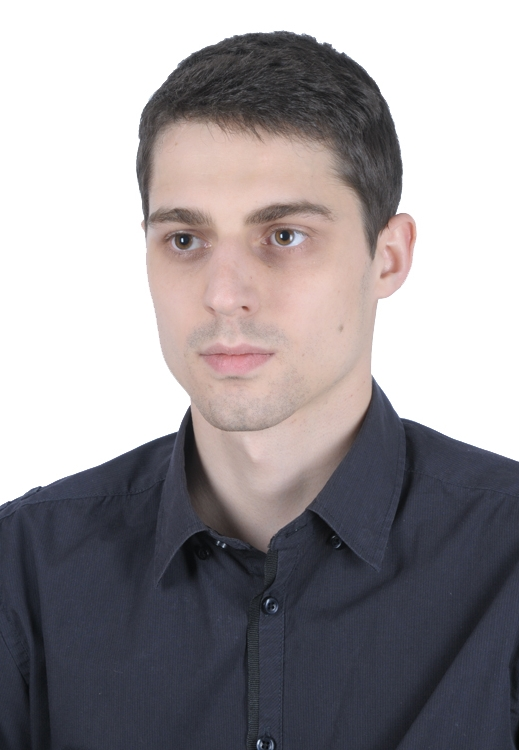
\includegraphics[width=\textwidth]{img/me-cv.jpg}
	\end{minipage}
	\hspace{0.5cm}
	\begin{minipage}[b]{0.6\textwidth}
		\begin{flushleft}
		Ireneusz Szulc
		
		{\it Kierunek:} Automatyka i Robotyka
		
		{\it Specjalność: } Informatyka przemysłowa
		
		{\it Urodzony:} 21. marca 1993~r. w Lublinie.
		
		{\it Numer indeksu:} 251001
		
		\end{flushleft}
	\end{minipage}
\end{figure}

Urodziłem się w Bździszewie.
W 2009 roku ukończyłem Gimnazjum w Woli Uhruskiej.
Następnie uczęszczałem do I Liceum Ogólnokształcącego im. Stefana Czarnieckiego w Chełmie.
W 2012 zdawałem maturę na poziomie rozszerzonym z matematyki i fizyki. 
Po maturze kontynuowałem naukę na Politechnice Warszawskiej na Wydziale Mechatroniki na kierunku Automatyka i Robotyka. 

\vspace{2cm}

\begin{flushright}
%bez wcięcia
	\noindent...................................
\end{flushright}